
\subsection{Stetige Wavelet-Transformation} 
Im Kapitel \ref{chapter:cwt} wurde die Theorie der Stetigen Wavelet-Transformation behandelt. In dieser Theorie haben wir gesehen das wir mit der Stetigen Wavelet-Transformation ein Zeit-Frequenz Analyse machen kann und gut interpretierbare Egebnisse erhält. Der Nachteil bei der cwt ist jedoch die grosse redundanz. Diese redundanz spiegelt sich in der Analysedauer wieder. Welsche schon bei simplen Datensätzen mehrere Sekunden dauern kann. Weshalb sie für eine realtime Applikation nicht geeignet ist.\\
Um dennoch die zu zeigen welche vorteile eine cwt bringen kann wurde noch einmal der Frequenzsweep \ref{fig:stftsig} mit einem Komplexen Gauss Wavelet Analysiert. Das komplexe Gauss-Wavelet ist wie folgt definiert:
\begin{equation}
\psi(t)=C \exp ^{-\mathrm{j} t} \exp ^{-t^{2}}
\end{equation}
Wobei $C$ eine Konstante ist. Das Komplexe Gauss Wavelet wird in der folgenden Analyse in der achten Ableitung verwendet. In der Python Library wird dies cgauN benennt wobei N für die häufigkeit der Ableitungen der Wavletfunktion steht.\\

Die Analyse wurde mit der Python Library pywt durchgeführt welche schon eine komplette cwt-Funktion bereitstellt. In der folgenden Abbildung \ref{fig:python-cwt} ist der wesentliche Ausschnitt aus dem Python Code dargestellt mit dem die cwt Analyse jeweils erstellt wurde. Da es sich um ein komplexes Wavelet handelt, wurde zur besseren veranschaulichung, die Absolutwerte der Analyse zur illustration verwendet.\\

\begin{figure}
	\centering
	\lstinputlisting[language=Python,firstline=9,lastline=26,numbers=left,style = Python]{papers/autotune/sections/frequenzanalyse/code/cwt.py}
	\caption{Python cwt Beispiel}
	\label{fig:python-cwt}
\end{figure}

Das Ergebnis der cwt ist in der Grafik \ref{fig:STFTCWT} ersichtlich. Dabei stehen sich eine STFT und cwt gegenüber. Dringend ist zu betrachten, dass dieser Vergleich auf keinsterweise eine allgemeingültige Aussage über diese zwei Arten der Zeit-Frequenz Analyse sein soll. Sondern mehr eine gegenüberstellung zur betrachtung von unterschieden. 

\begin{figure}[!ht]
	\centering
	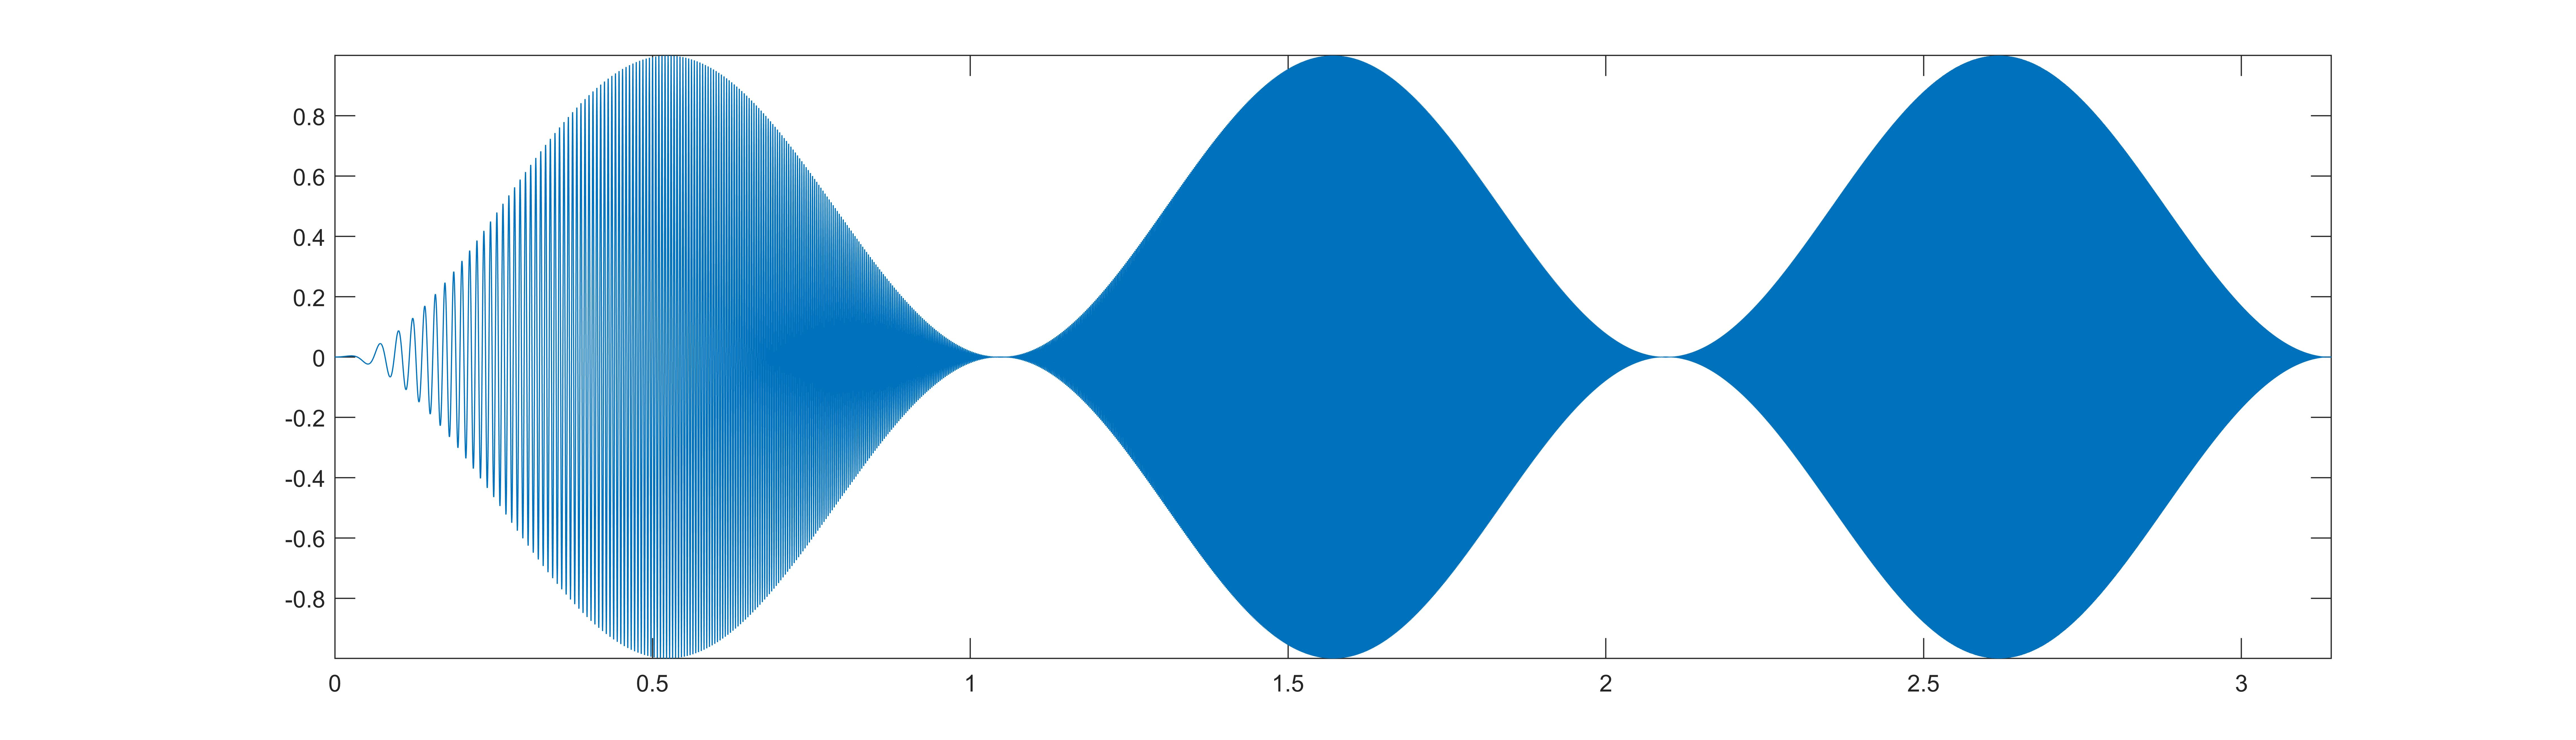
\includegraphics[width=\linewidth]{papers/autotune/sections/fft/signal.jpg}
	\captionof{figure}{Sweep Signal 0-400$Hz$}\label{fig:stftsig}
	\begin{tabularx}{\columnwidth}{XX}
		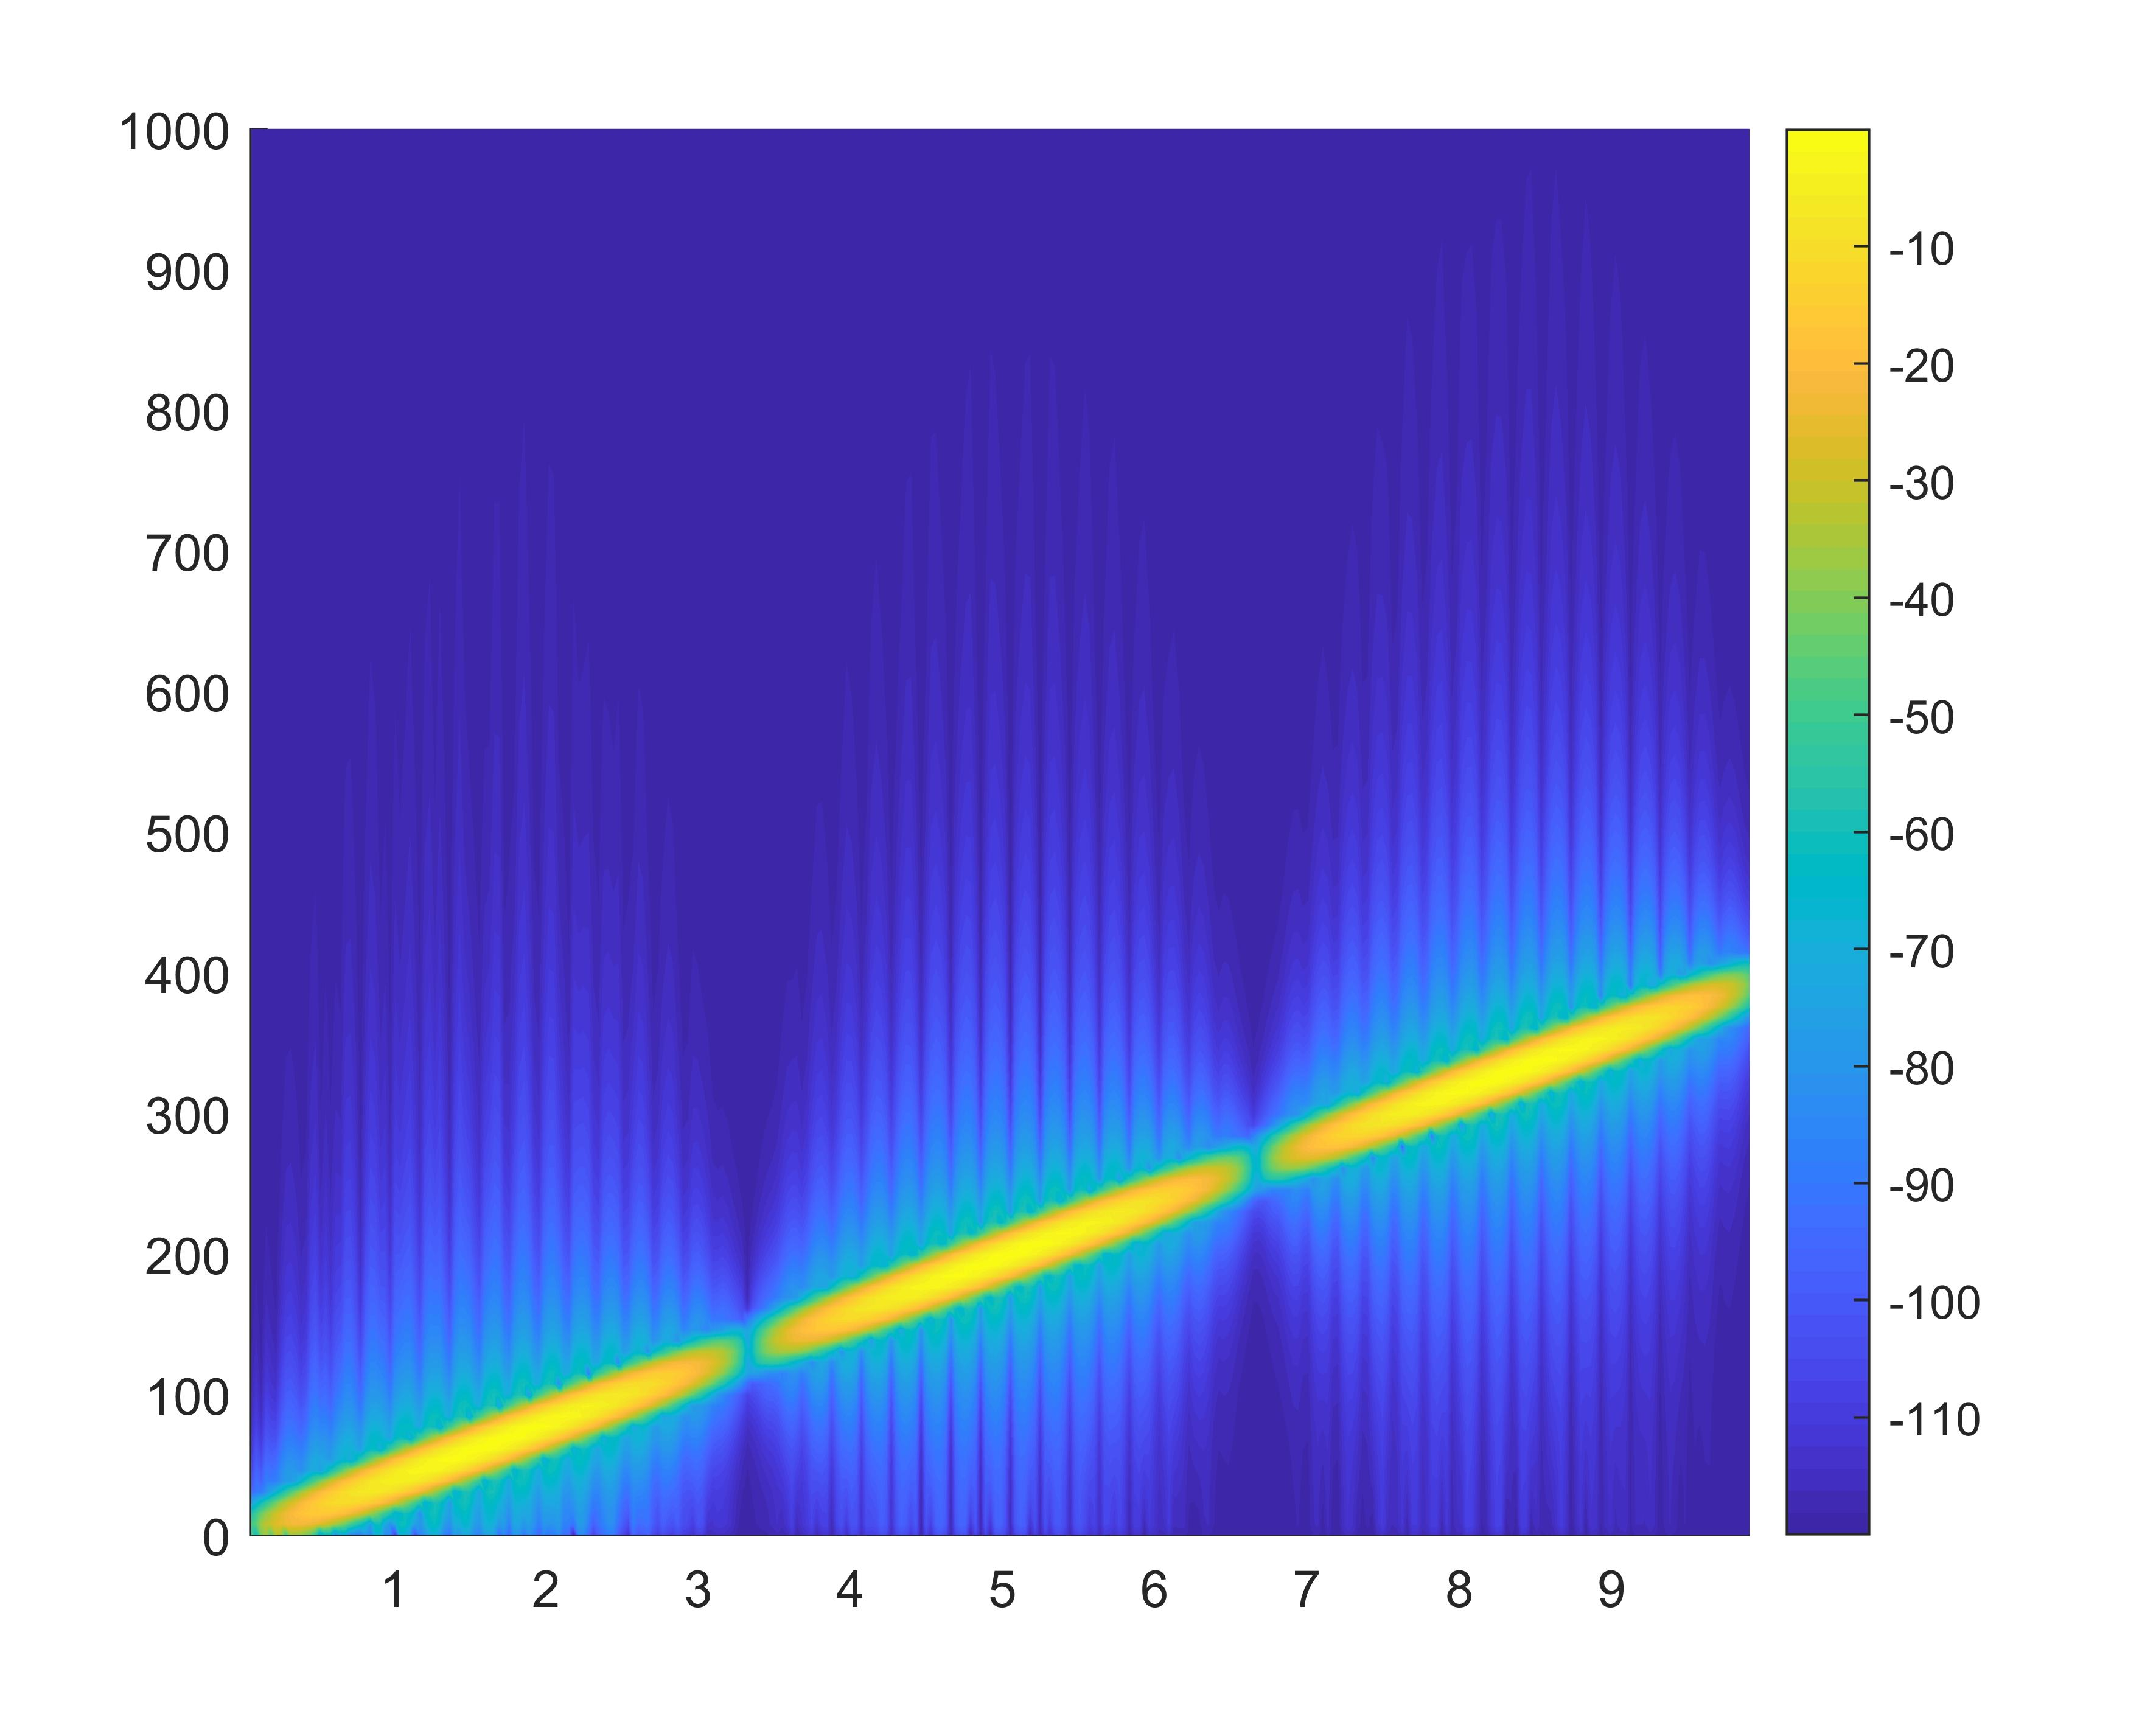
\includegraphics[width=\linewidth]{papers/autotune/sections/fft/stft4096.jpg}
		\captionof{figure}{STFT Blackman mit 4096 Sample Fenster}\label{fig:stft256}
		&   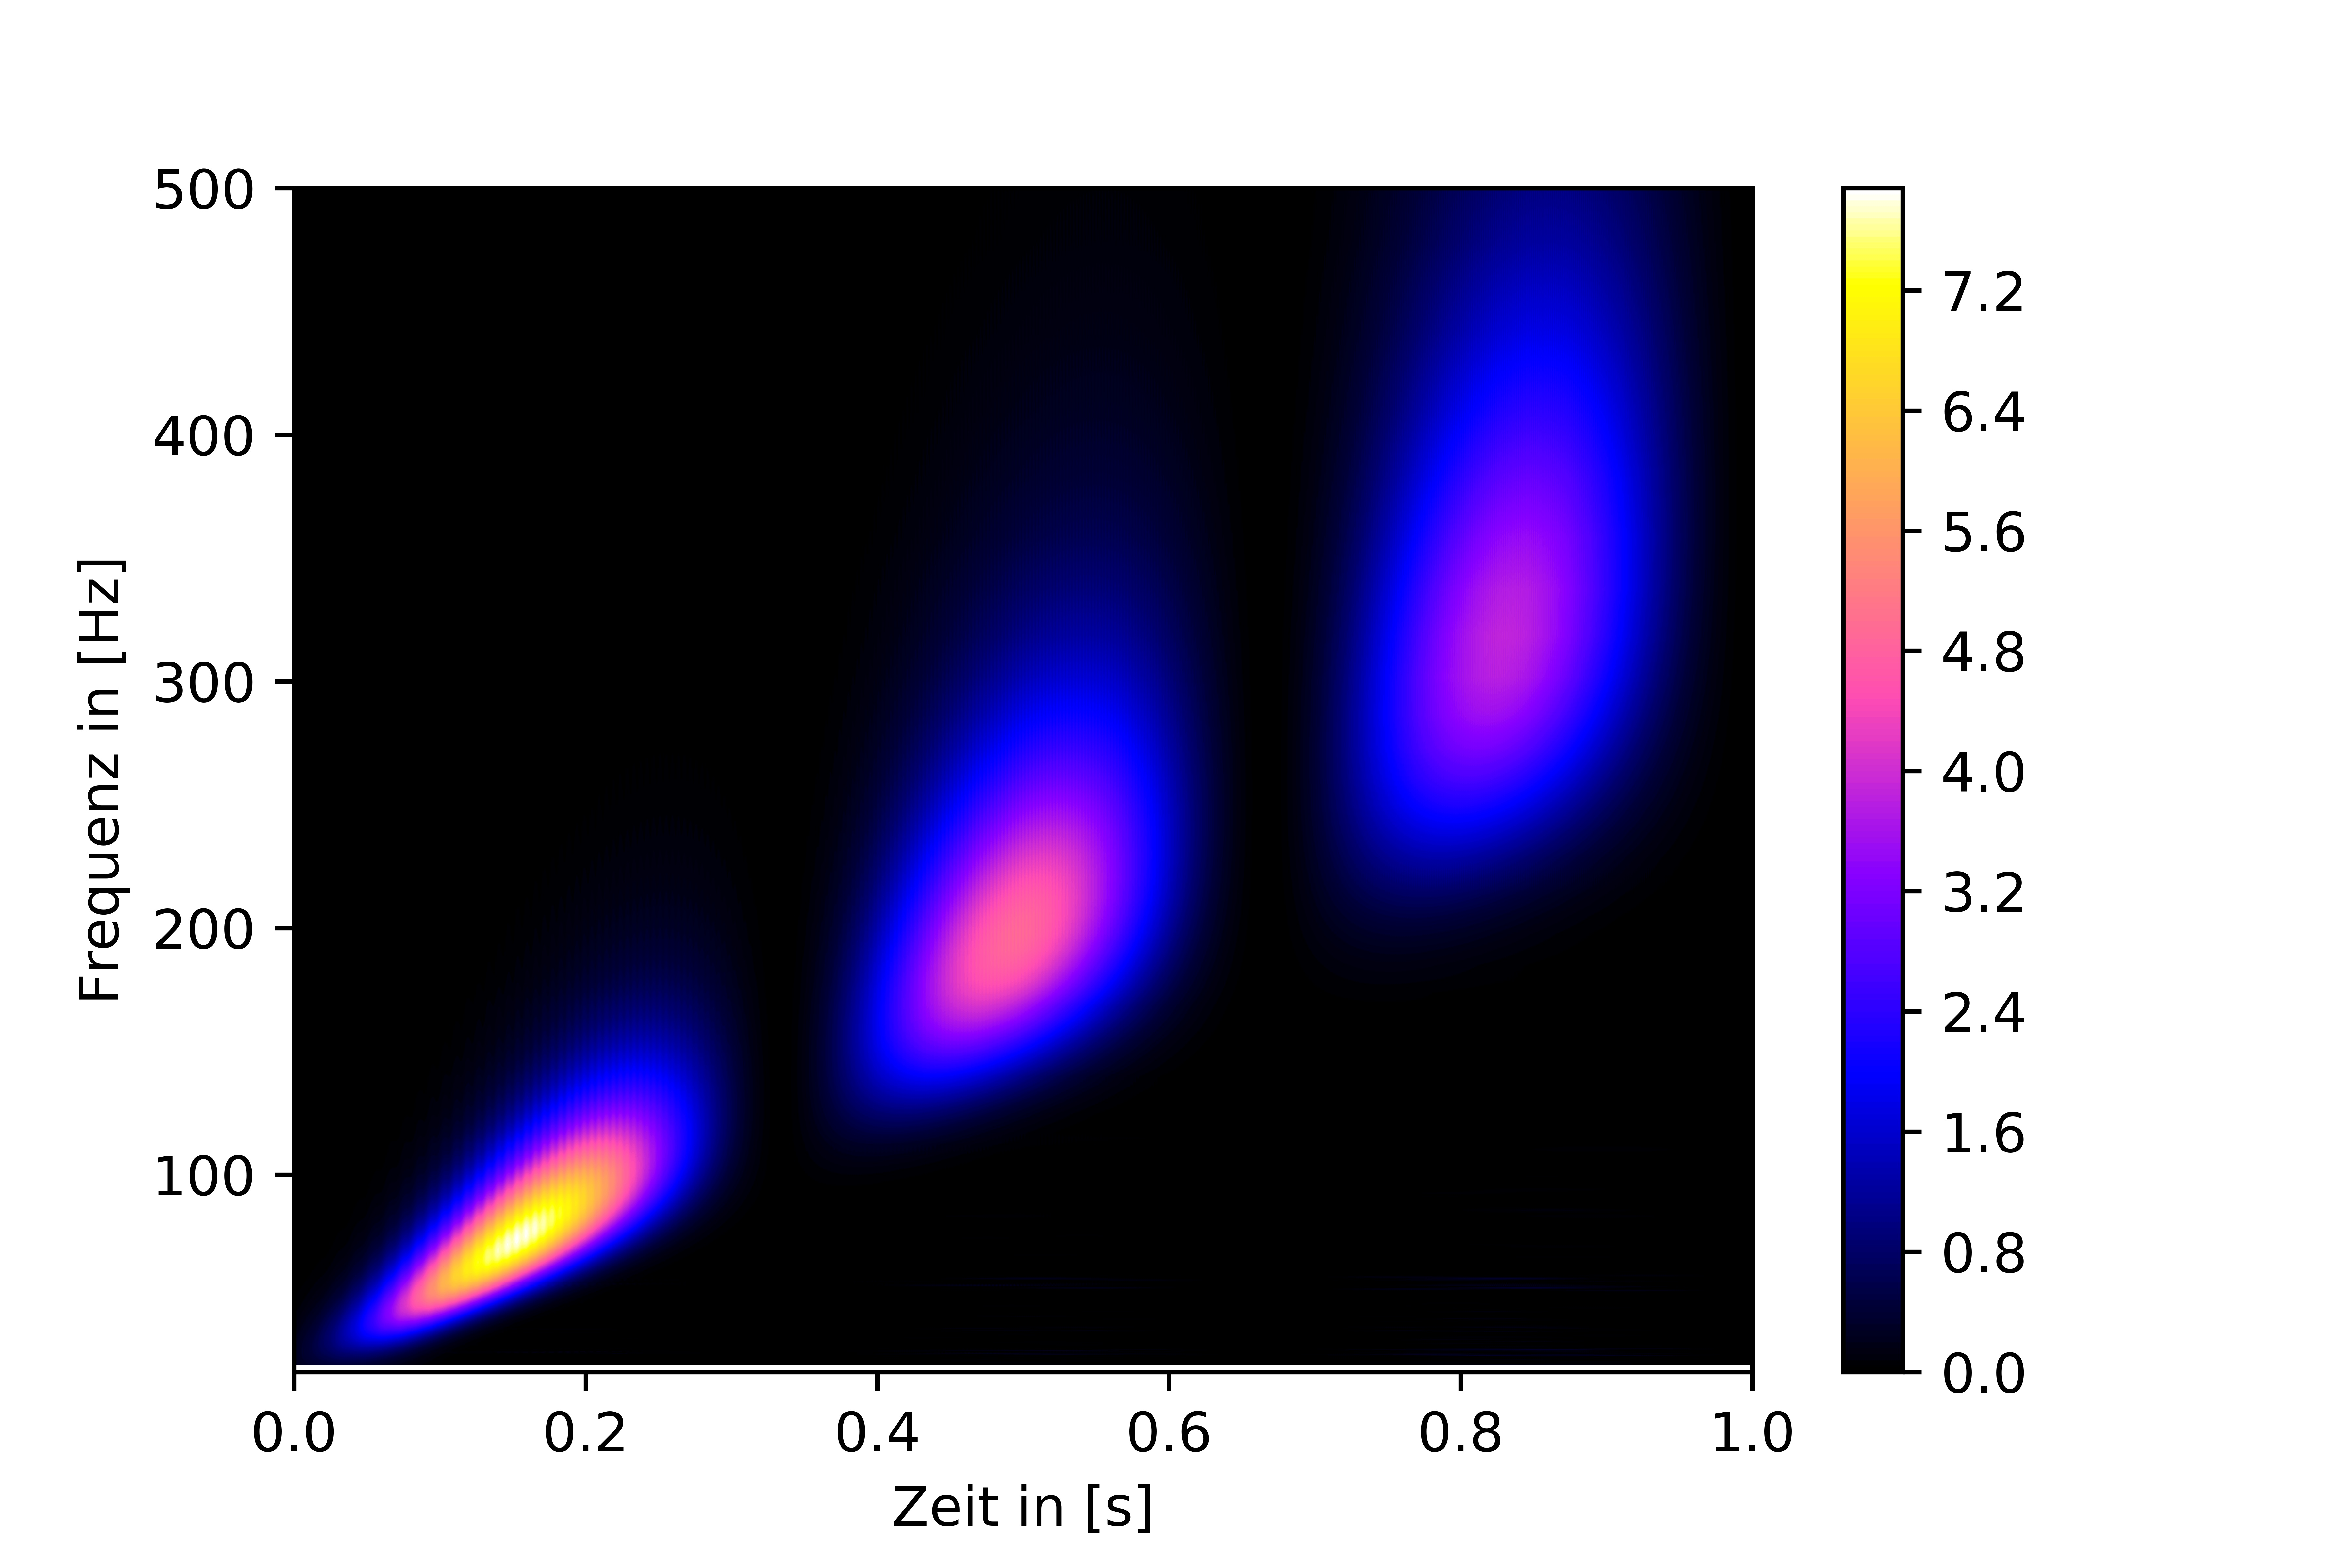
\includegraphics[width=1.24\linewidth]{papers/autotune/sections/frequenzanalyse/images/sinsweep.jpg}   
		\captionof{figure}{Dauberchi 8 Cwt Analyse des Frequensweeps}\label{fig:cwtsweep}         
	\end{tabularx}
	\caption{figure}{Vergleich zwischen STFT und der CWT}
	\label{fig:STFTCWT}
\end{figure}%


\subsection{Diskrete Wavelet-Transformation}
Die diskrete Analyse ... hier noch eine gute einleitung

\begin{figure}[!ht]
	\centering
	\scalebox{.75}{
		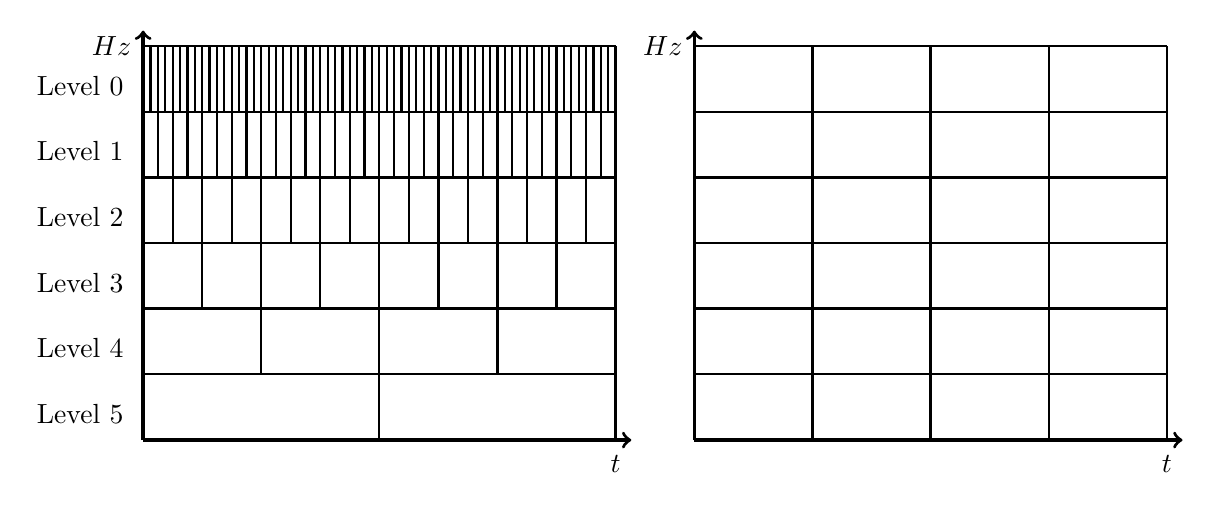
\begin{tikzpicture}
		\draw (6,-5.3) node{$t$};
		\draw (-0.4,0) node{$Hz$};
		
		\draw (-0.8,-0.5) node{Level 0};
		\draw (-0.8,-1.333) node{Level 1};
		\draw (-0.8,-2.166) node{Level 2};
		\draw (-0.8,-2.999) node{Level 3};
		\draw (-0.8,-3.832) node{Level 4};
		\draw (-0.8,-4.665) node{Level 5};
		
		
		\draw[->, very thick] (0,-5)--(0,0.2);
		\draw[->, very thick] (0,-5)--(6.2,-5);
		
		\draw[thick] (0,-0)--(6,-0);
		\draw[thick] (0,-0.833)--(6,-0.833);
		\draw[thick] (0,-1.666)--(6,-1.666);
		\draw[thick] (0,-2.499)--(6,-2.499);
		\draw[thick] (0,-3.33)--(6,-3.33);
		\draw[thick] (0,-4.166)--(6,-4.166);
	
		\draw[thick] (3,-5)--(3,0);
		\draw[thick] (6,-5)--(6,0);
		\draw[thick] (1.5,-4.166)--(1.5,0);
		\draw[thick] (4.5,-4.166)--(4.5,0);
		
		\draw[thick] (0.75,-3.33)--(0.75,0);
		\draw[thick] (2.25,-3.33)--(2.25,0);
		\draw[thick] (3.75,-3.33)--(3.75,0);
		\draw[thick] (5.25,-3.33)--(5.25,0);
		
		\foreach \x in {0,0.375,...,6}
			\draw[thick] (\x,-2.499)--(\x,0);
		
		\foreach \x in {0,0.1875,...,6}
			\draw[thick] (\x,-1.666)--(\x,0);
		
		\foreach \x in {0,0.09375,...,6}
			\draw[thick] (\x,-0.833)--(\x,0);
		
		\draw (13,-5.3) node{$t$};
		\draw (6.6,0) node{$Hz$};
		\draw[->, very thick] (7,-5)--(7,0.2);
		\draw[->, very thick] (7,-5)--(13.2,-5);
		
		\draw[thick] (7,-0)--(13,-0);
		\draw[thick] (7,-0.833)--(13,-0.833);
		\draw[thick] (7,-1.666)--(13,-1.666);
		\draw[thick] (7,-2.499)--(13,-2.499);
		\draw[thick] (7,-3.33)--(13,-3.33);
		\draw[thick] (7,-4.166)--(13,-4.166);
		
		\draw[thick] (8.5,-5)--(8.5,0);
		\draw[thick] (10,-5)--(10,0);
		\draw[thick] (11.5,-5)--(11.5,0);
		\draw[thick] (13,-5)--(13,0);
		\end{tikzpicture}
	}
	\caption{Multiskalenanalyse Auflösung im Vergleich zu STFT Analyse}\label{fig:faauf}
	
\end{figure}

Wie man in der Abbildung \ref{fig:faauf} erkennt übernimmt einem die Multiskalenanalyse das Fenstern. Dabei geht die Wavelet-Transformation einen Kompromiss ein. Im oberen bereich bei den schnelleren Frequenzen sieht man den Zeitpunkt sehr genau. Die tiefen Frequenzen werden dabei wie bei einem Hochpass weggefiltert. In den tieferen Levels sieht man aber trozdem noch die Tiefen Frequenzen. Jedoch sind diese nicht mehr sehr genau auf dem Zeitstrahl abgebildet. Gerade bei der Multiskalenanalyse können durch tiefe Frequenzen an den Rändern oder Sprüngen eines Signales Artifkten enstehen. In der Grafik \ref{fig:faauf} können die beiden Darstellungen der Zeit-Frequenzaufteilung von der STFT und Diskreten Wavelet-Transformation nicht direkt miteinander verglichen werden sondern dienen zur Sinnbildlichen darstellung in dessen Aufteilung\\

Um dies zu verdeutlichen wird eine  Multiskalenanalyse des gleichen Sinussweepes gemacht wie in der Grafik \ref{fig:STFT} und gleich mit der STFT verglichen.
Die msa wird mit dem Dauberchie 8 Wavelet durchgeführt welches auch in der folgenden Tabelle \ref{tab:Dauberchies} über die Dauberchies Familie zu finden ist. Die diskrete Analyse kann nicht mit dem gleichen Wavelet durchgeführt werden da in der Python pywt Library die Stetigen und Diskreten Wavelets getrennt sind und es keine Überlappungen gibt. \\
In dieser Tabelle \ref{tab:Dauberchies} werden vier verschiedene Dauberchies Wavelets in verschiedner Auflösung dargestellt. Aus der Tabelle sind die Numerisch berechneten Vater und Mutter Wavelets der Dauberchien Reihe. Auch wird gut ersichtlich das die höheren Dauberchiesfunktionen mehr Samples brauchen um korrekt dargestelltzu werden.Zur berechnung der Koeffizienten wird auf das Kapitel \ref{chapter:daubechies} verwiesen.\\

\begin{table}
	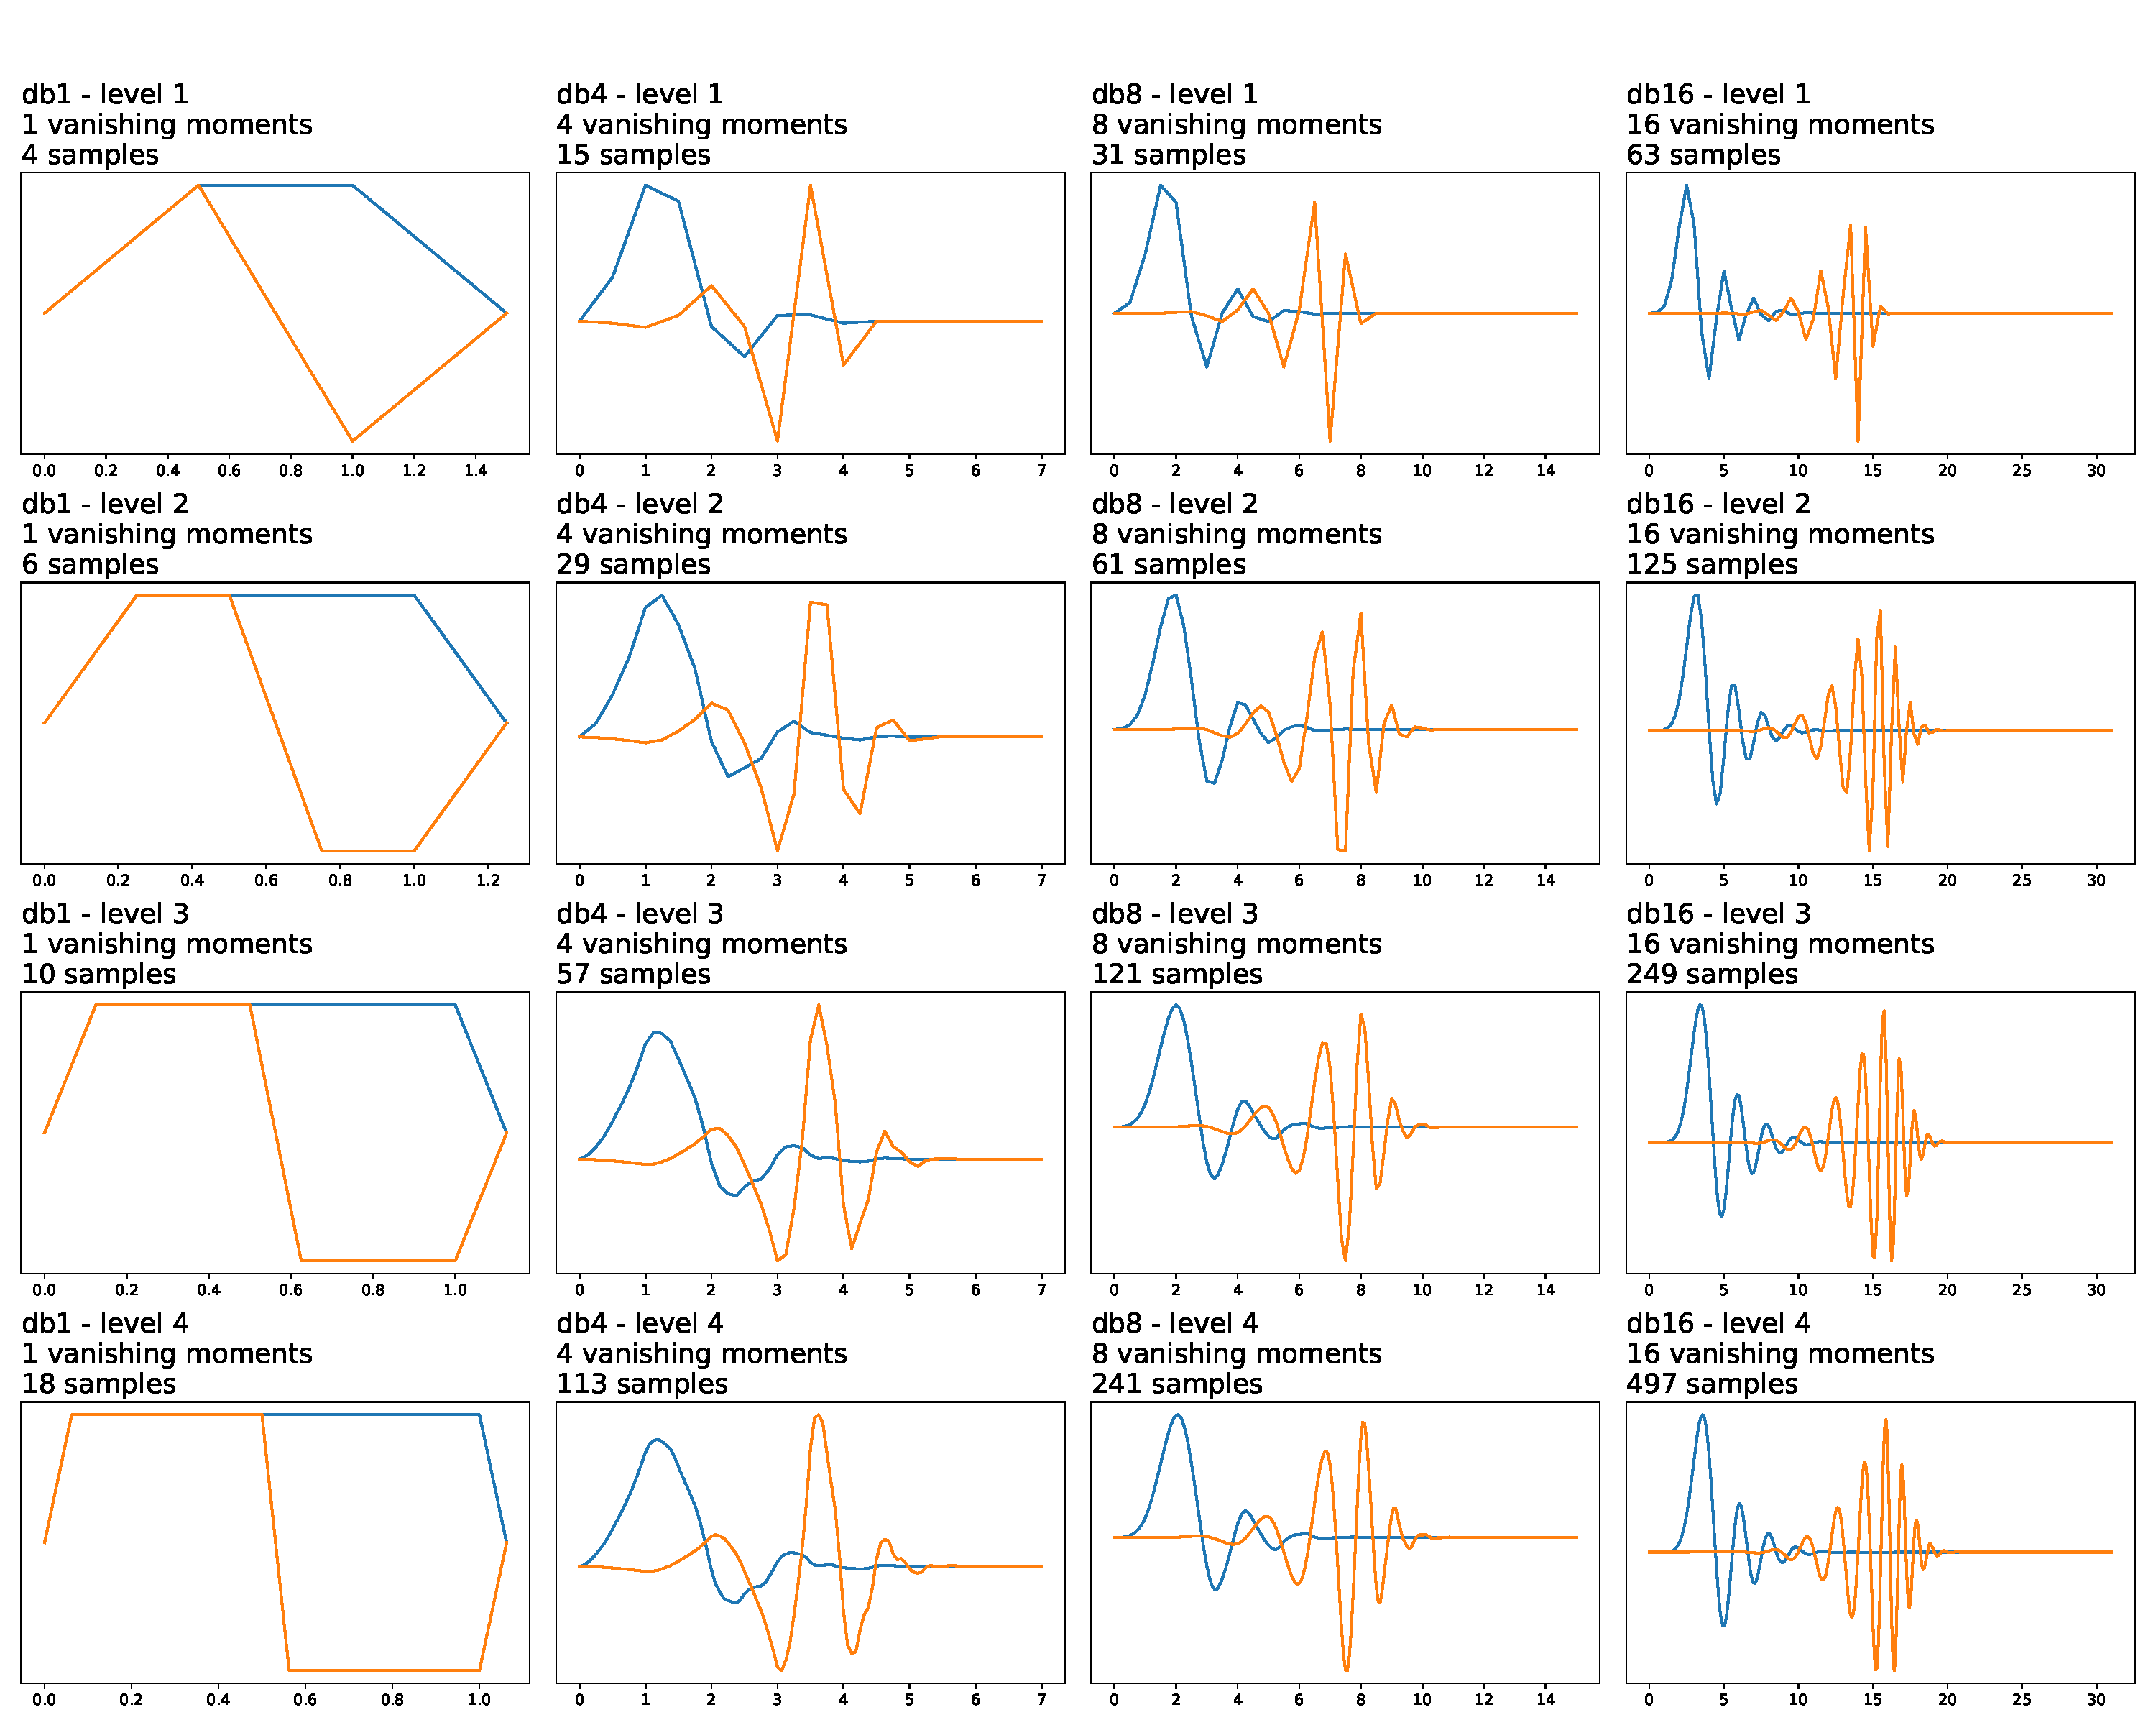
\includegraphics[width=\linewidth]{papers/autotune/sections/frequenzanalyse/images/DauberchiesFamilie.pdf}
	\caption{Eine kleine Auswahl aus der Dauberchies Familie}
	\label{tab:Dauberchies}
\end{table}

Das Ergebnis der Diskreten Wavelet-Tranformation ist in der Grafik \ref{fig:sin-sweep} wiedergegeben. Man sieht eine klare verschlechterung der Ergebnisse im vergleich mit der cwt Analyse aus \ref{fig:STFTCWT} im Frequenzbereich. Man erkennt nur die jeweiligen Oktaven die in der Zeit dargestellt werden. Für eine genauere Analyse sind diese ergebnisse jedoch unbrauchbar.  

\begin{figure}[!ht]
	\centering
	\includegraphics[width=\linewidth]{papers/autotune/sections/frequenzanalyse/images/sweepdwt.jpg}
	\captionof{figure}{Diskrete Wavelet Analyse des Sinus Sweep 0-400$Hz$}\label{fig:sin-sweep}
\end{figure}%


\newpage

